\section{State of the Art}
This chapter reviews recent advances in robot skill acquisition and perception, focusing on two complementary research lines. The first is Programming by Demonstration (PbD), which reduces the barrier for end-users to teach robots by allowing skills to be transferred through demonstration rather than explicit coding. The second is six-degree-of-freedom (6D) pose estimation, which provides robots with the perception capabilities required to interact robustly with objects in unstructured environments. Taken together, these topics represent two essential pillars of autonomy: intuitive skill transfer and reliable scene understanding. The chapter is structured as follows: Section~\ref{subsec:pbd} discusses classical and AR-assisted PbD approaches, while Section~\ref{subsec:pose} surveys classical, AI-assisted, and fully AI-based methods for 6D pose estimation.

\subsection{Programming by Demonstration (PbD)}
\label{subsec:pbd}

Programming by Demonstration (PbD) is an approach that enables robots to acquire skills by observing or experiencing a task instead of relying on explicit coding \cite{calinon2009robot}. The roots of this field lie in early work by Lozano-Perez on spatial planning and robot programming environments \cite{lozano1983spatial}, which highlighted the need for intuitive methods that make robot programming feasible for non-experts. Over time, PbD has become an important paradigm both in robotics and in human–computer interaction, with notable contributions spanning kinesthetic teaching, teleoperation, and dialog-based learning \cite{friedrich1996robot,calinon2009robot}.

Figure~\ref{fig:pbd_classical} illustrates the concept of PbD. On the left, kinesthetic teaching is shown, where a human physically guides the robot’s arm through the task. On the right, reproduction is depicted, in which the robot performs the trajectory observed in the demonstration \cite{calinon2007learning}.

\begin{figure}[H]
    \centering
    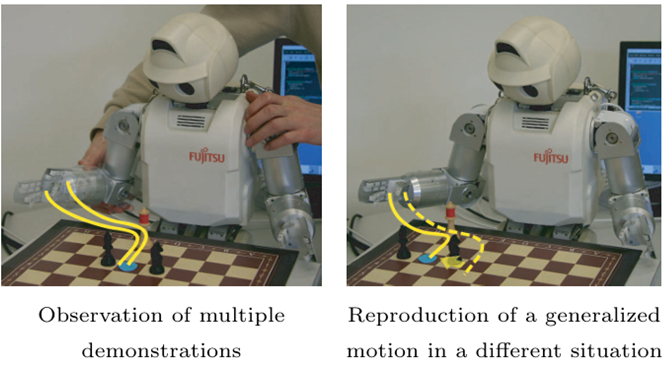
\includegraphics[width=\textwidth]{figures/pbd.png}
    \caption[Programming by Demonstration: kinesthetic teaching and reproduction]{Programming by Demonstration: kinesthetic teaching (left) and task reproduction (right) \cite{calinon2007learning}.}
    \label{fig:pbd_classical}
\end{figure}

\subsubsection{Principles of Classical PbD}

At its core, PbD transfers task knowledge either through direct physical interaction with the robot or by recording human demonstrations with external devices. Two dominant paradigms characterize the classical approaches.  

In \emph{kinesthetic teaching}, the operator physically moves the robot manipulator along the desired trajectory. This direct guidance enables the robot to record the motion in real time, and collaborative robots make this process easier by providing backdrivable joints through integrated torque sensors.  

In contrast, \emph{teleoperation} relies on external input devices such as joysticks, six-degree-of-freedom (6D) mice, or haptic interfaces. In this setup, the operator remotely controls the robot while the system records end-effector poses or joint trajectories.  

Both approaches ultimately generate motion sequences—whether in joint space or task space—along with discrete commands such as grasping or releasing actions \cite{friedrich1996robot}.  

\paragraph{Classical Demonstration Pipeline} Early implementations of Robot Programming by Demonstration (RPD) were typically organized into two broader phases: (1) demonstration, analysis, and induction, and (2) completion and execution \cite{friedrich1996robot}. Figure~\ref{fig:pbd_pipeline} illustrates this process in detail.  

In the first phase, the user demonstrates the task on the robot system. The analyzer then segments and standardizes the recorded motions, which are further processed by an induction unit to generalize or specialize the behavior. The results are stored as a sequence of basic operations in a knowledge base.  

In the second phase, the planning system retrieves this knowledge to assemble a skeleton program for the desired task. With feedback from the user, this program is completed into a full sequence of basic operations. An interpreter translates the program into executable commands, which are then carried out by the robot system.  

The figure highlights how the user remains integrated into both phases, shown by dashed arrows, ensuring that ambiguities in the demonstration are resolved interactively.  

\begin{figure}[H]
    \centering
    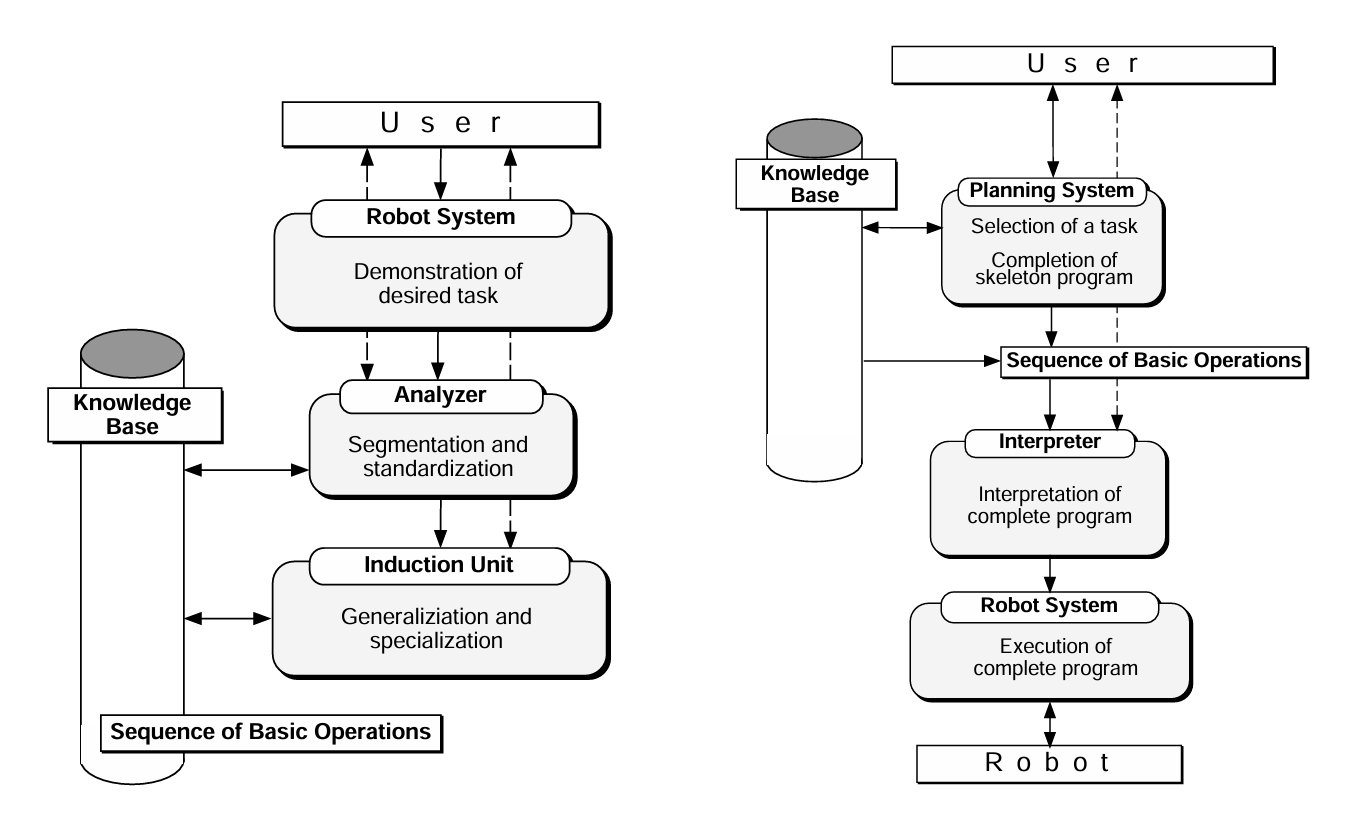
\includegraphics[width=0.8\textwidth]{figures/pbd_pipeline.png}
    \caption[Classical RPD process]{Phase~1 (demonstration, analysis, and induction) and Phase~2 (completion and execution) of the RPD process. Dashed arrows indicate the integration of the user \cite{friedrich1996robot}.}
    \label{fig:pbd_pipeline}
\end{figure}

\paragraph{Strengths, Limitations, and Advances}
Classical PbD represented a major step forward compared to low-level teach-in programming because it significantly reduced the complexity of programming robots for everyday users. At the same time, several limitations became apparent as these systems were tested in practical contexts \cite{friedrich1996robot}.  

One of the central challenges was generalization. Demonstrations often applied only to the exact scenario that was shown, and extending a learned behavior to variations in the task—such as objects in different positions or with different shapes—proved difficult. Data scarcity further reinforced this problem, as only a handful of demonstrations were usually available, making it hard for the system to infer robust task models from limited input.  

Another limitation was the reliance on sensors. Early PbD implementations required specialized or expensive hardware for motion capture, and their adaptability to dynamic or cluttered environments was limited. Furthermore, the human effort required could be significant. Kinesthetic teaching demanded physically guiding the robot arm, which could be exhausting for longer tasks, while teleoperation often suffered from precision bottlenecks introduced by the input devices.  

To address these issues, later research introduced probabilistic methods that explicitly model variability and uncertainty in demonstrations \cite{calinon2009robot}. Gaussian Mixture Models (GMMs) and Hidden Markov Models (HMMs) allowed the system to capture distributions over trajectories instead of memorizing single paths. This provided a way to generalize beyond the demonstrated task by identifying invariant features, such as grasping any object of a certain shape rather than only the one used during training.  

Probabilistic modeling also enabled systems to handle noise and inconsistencies in demonstrations by assigning higher weight to likely trajectories while ignoring outliers. In addition, these methods allowed adaptation to new contexts by conditioning the learned model on external variables such as object positions or environmental constraints. By combining robustness with flexibility, probabilistic approaches built directly upon the foundations of classical PbD while overcoming many of its inherent weaknesses.

\subsubsection{AR-Assisted Approaches}

Augmented Reality (AR) enhances PbD by providing intuitive interfaces for task instruction. Using AR headsets or tablets, users can demonstrate tasks naturally without programming expertise \cite{andersson2016ar}. Soares et al.\ \cite{soares2021programming} proposed a complete AR-based system enabling non-experts to program collaborative and industrial robots via hand gestures captured through Microsoft HoloLens~2. Their approach divides the system into two subsystems: an AR interface for recording gestures and a backend translator that converts the recorded paths into robot-specific code (URScript for UR5 and RAPID for ABB IRB~2600).

The AR interface, built in Unity and deployed on the HoloLens~2, tracks hand movement via gestures (e.g., Air Tap) and allows the user to define coordinate systems and visualize the robot's reachable workspace. Once recorded, hand trajectories are sent using the tools of Robot Operating System (ROS) \cite{osrf_ros} to a translator node that reorients the coordinates (to match robot frames) and generates robot programs.

Testing involved instructing both robots to trace geometric shapes such as triangles and squares. For example, the UR5 was successfully able to replicate a triangle drawn in space (Figure~\ref{fig:ur5_triangle}), and the ABB IRB~2600 performed a more complex 3D path as shown in Figure~\ref{fig:abb_3d_path}.

\begin{figure}[H]
  \centering
  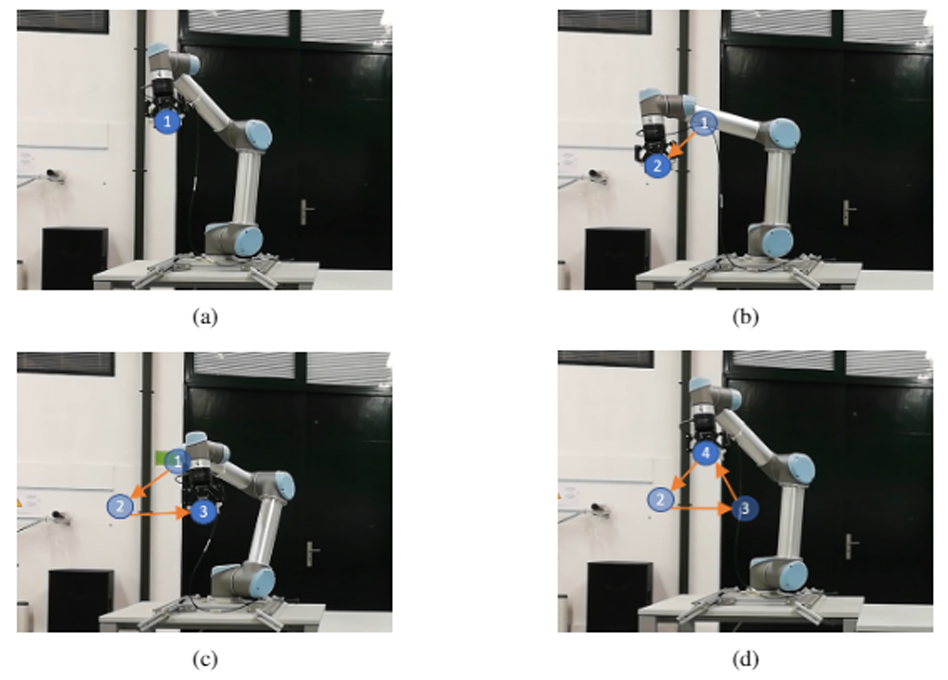
\includegraphics[width=\textwidth]{figures/URP_path_triangle.png}
  \caption[UR5 path execution (triangle)]{UR5 path execution (triangle): (a) robot at initial point, (b) robot at second point, (c) robot at third point, (d) robot at final point \cite{soares2021programming}.}
  \label{fig:ur5_triangle}
\end{figure}

\begin{figure}[H]
  \centering
  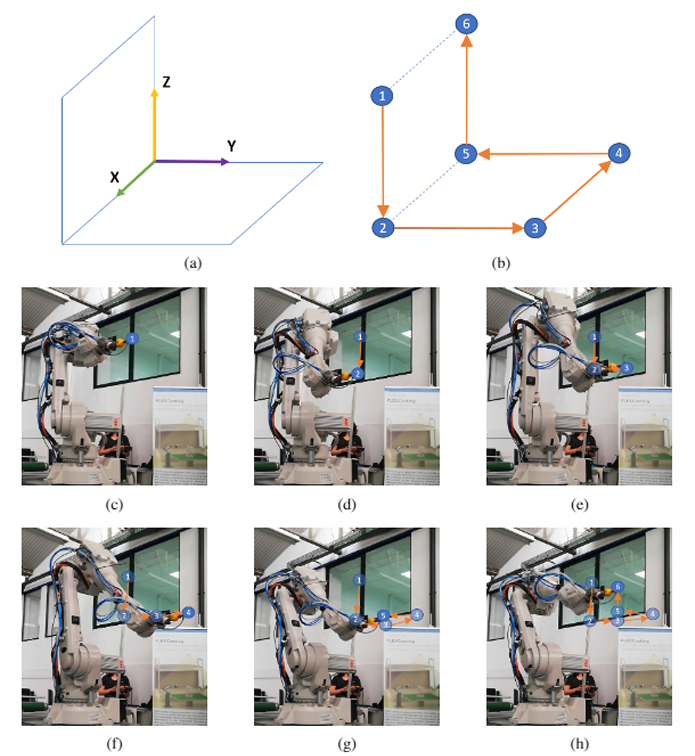
\includegraphics[width=\textwidth]{figures/ABB_IRB_3d_path.png}
  \caption[ABB IRB~2600 3D path execution]{ABB IRB~2600 path execution (3D solid): (a) path referential frame, (b) path sequence, (c) robot at initial point, (d) robot at second point, (e) robot at third point, (f) robot at fourth point, (g) robot at fifth point, (h) robot at final point \cite{soares2021programming}.}
  \label{fig:abb_3d_path}
\end{figure}

In all cases, path replication errors ranged between 1--3~cm, which is acceptable for low-precision industrial tasks \cite{soares2021programming}.

Lotsaris et al.\ \cite{lotsaris2021ar} extended the concept of AR-based PbD by developing a complete, ROS-integrated system for industrial robot programming using Microsoft HoloLens. Their objective was to create a tool that allows non-expert users to program robots intuitively by manipulating a virtual end-effector (gripper) directly in 3D space. The system was designed with a strong emphasis on usability, simplicity, and responsive feedback.

\begin{figure}[H]
  \centering
  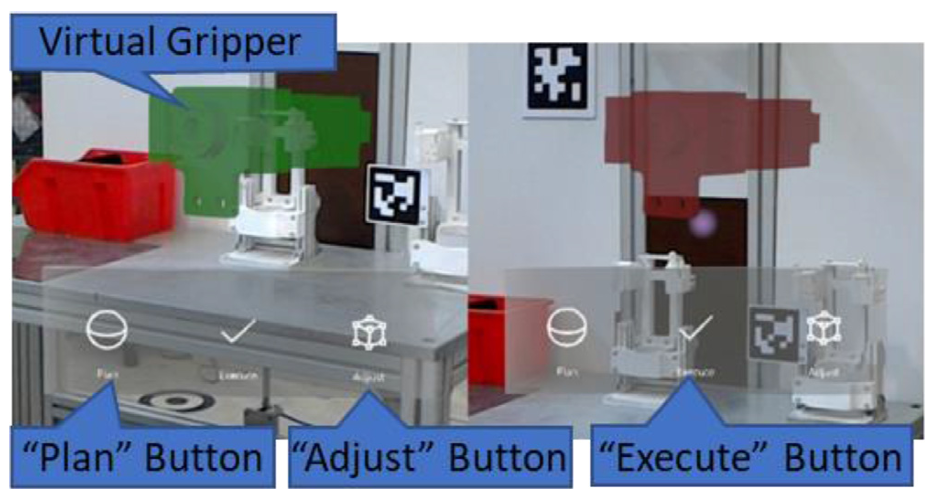
\includegraphics[width=0.9\textwidth]{figures/gripper_feedback_ui.png}
  \caption[Visual feedback for trajectory planning]{Visual feedback for trajectory planning: left (success), right (failure) \cite{lotsaris2021ar}.}
  \label{fig:plan_feedback}
\end{figure}

The interface shown in Figure~\ref{fig:plan_feedback} presents a virtual gripper with minimal user interface that contains three buttons: \textit{Rotate}, \textit{Plan}, and \textit{Execute}. Users manipulate the gripper by moving the control points shown in Figure~\ref{fig:hololens_interface} using air gestures (e.g., Air Tap and Drag) and can generate motion plans for the robot by positioning the gripper and clicking the \textit{Plan} button. If the plan is successful, the gripper turns green; if it fails, it turns red.

\begin{figure}[H]
  \centering
  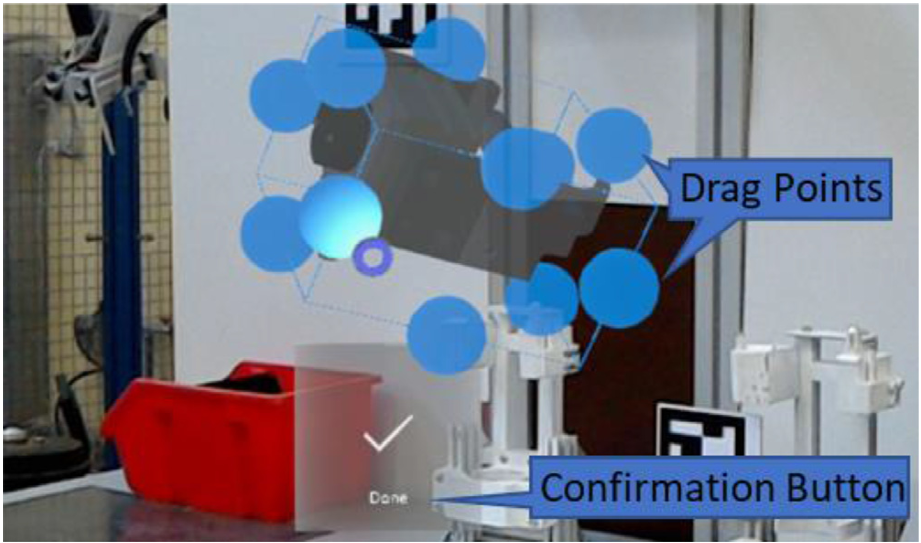
\includegraphics[width=0.8\textwidth]{figures/gripper_rotate_ui.png}
  \caption[HoloLens AR interface with virtual gripper]{AR interface in HoloLens showing the virtual gripper and its pose control points \cite{lotsaris2021ar}.}
  \label{fig:hololens_interface}
\end{figure}

\textit{Coordinate calibration and integration:} A critical step in the system involves aligning the AR and robot coordinate frames. To accomplish this, the system uses a QR-code-based initialization phase. The HoloLens captures an image of a known marker placed near the robot base; the system then computes the transformation between AR and robot frames. Once the transformation is established, user-defined gripper poses in AR space are transformed and transmitted to ROS. Motion planning and execution are then handled by MoveIt \cite{sucan_moveit}, and trajectory feedback is sent back to the AR device for visualization.

\textit{Evaluation and results:} The system was tested in a case study involving front suspension assembly in the automotive sector. Operators used the application for:
\begin{enumerate}
    \item \textbf{Teaching:} Defining new waypoints and poses for assembly.
    \item \textbf{Error recovery:} Repositioning the robot quickly in response to execution errors or dynamic changes.
\end{enumerate}

Results showed that the application allowed fast and intuitive robot instruction with no programming experience. The AR visualization of planned paths (Figure~\ref{fig:trajectory_preview}) prevented unsafe or unreachable motions, thus reducing downtime and error rates \cite{lotsaris2021ar}.

\begin{figure}[H]
  \centering
  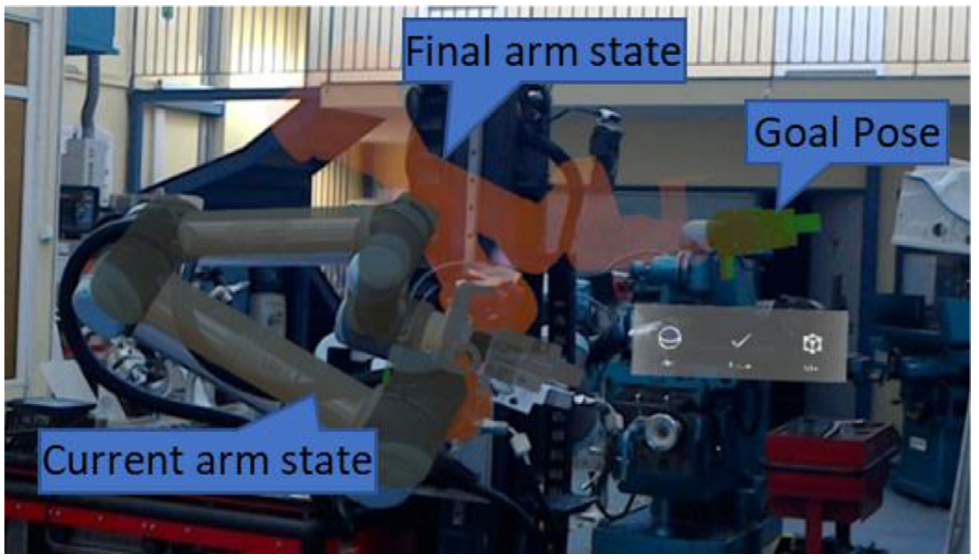
\includegraphics[width=\textwidth]{figures/trajectory_planning.png}
  \caption[AR trajectory preview for planned motions]{Trajectory preview via AR showing path planning before execution \cite{lotsaris2021ar}.}
  \label{fig:trajectory_preview}
\end{figure}

\textit{Limitations and future work:} Despite its benefits, the system has some limitations:
\begin{itemize}
    \item QR-code-based calibration lacks sub-centimeter precision.
    \item HoloLens ergonomics limit prolonged use.
\end{itemize}
Future improvements aim to support multi-robot configurations, expand task domains (e.g., drilling, sanding), and integrate better safety validation. The modular ROS architecture makes it adaptable to other platforms, promoting generalizability. This work illustrates a mature AR-assisted PbD system validated in a real industrial context, showing strong potential for deployment in flexible and reconfigurable manufacturing environments \cite{lotsaris2021ar}.

\subsection{6D Pose Estimation}
\label{subsec:pose}

6D pose estimation refers to determining an object’s position and orientation in 3D space, which is a crucial step for manipulation and interaction tasks \cite{thalhammer2024challenges}. This section compares classical, AI-assisted, and fully AI-based approaches for 6D pose estimation.

\subsubsection{Classical Approaches}

Classical 6D pose estimation methods rely on geometric alignment and handcrafted features rather than learned representations. Template-based approaches render CAD models from many viewpoints and match them to query images, which makes them naturally robust to symmetries but computationally expensive when scaling to large object sets. Feature-based techniques align edges or local descriptors with 3D models and work reliably under controlled conditions, yet they quickly degrade in cluttered or occluded scenes. Depth-based methods, often coupled with Iterative Closest Point (ICP), refine poses by aligning observed point clouds to object models, though they require accurate depth sensing and fail on reflective or transparent objects \cite{thalhammer2024challenges}.  

Building on this tradition, Hwang et al.\ developed an efficient non-AI-assisted ICP enhancement algorithm for 6D pose tracking of household objects \cite{hwang2025icp}. Their approach integrates coarse registration using keypoints tracked with the Kanade–Lucas–Tomasi (KLT) method \cite{lucas1981iterative}, refinement with a weighted point-to-plane metric to handle symmetries and flat objects, and validation with recovery to address tracking failures. Figure~\ref{fig:pose_classical} summarizes the overall process.

\begin{figure}[H]
    \centering
    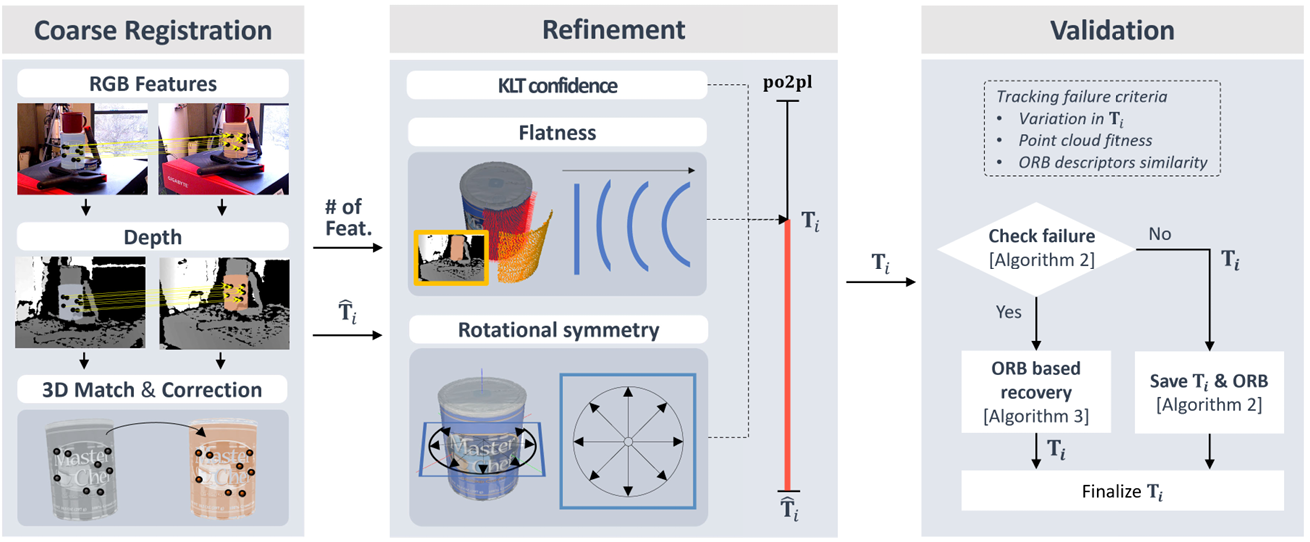
\includegraphics[width=\textwidth]{figures/6destimationKLT.png}
    \caption[ICP-based 6D pose tracking with KLT keypoints]{ICP enhancement algorithm: coarse registration from KLT keypoints \cite{lucas1981iterative} and depth, refinement with a weighted point-to-plane metric for symmetry and flatness, and validation with recovery for tracking failures \cite{hwang2025icp}.}
    \label{fig:pose_classical}
\end{figure}

\subsubsection{AI-Assisted Approaches}
\label{subsubsec:aiassisted}

AI-assisted pipelines often integrate deep learning for detection or segmentation with geometry-based pose estimation. A research team at the Technical University of Munich (TUM) has made several contributions in this area, as well as in fully AI-based approaches \cite{manhardt2020cps++,wang2020self6d,wang2021occlusion,di2021so}. Among them, CPS++ \cite{manhardt2020cps++} provides an end-to-end framework for monocular, class-level 6D pose estimation with metric shape recovery.

The method jointly regresses 6D pose, metric scale, and a low-dimensional shape embedding from a single RGB image. Based on a two-stage design, objects are first localized with RetinaNet \cite{del2021retinanet}, then each region of interest is processed by a \emph{lifter} module that predicts pose and shape parameters. Shapes are reconstructed through class-specific AtlasNet decoders \cite{vakalopoulou2018atlasnet}, yielding dense point clouds and meshes. Training relies on synthetic data from ShapeNet \cite{chang2015shapenet}, while the CPS++ extension introduces a self-supervised loss to bridge the synthetic-to-real gap without annotated labels.

Figure~\ref{fig:qual_real} illustrates the approach: from a monocular RGB input, CPS++ detects unseen objects, estimates their 6D pose and metric scale, reconstructs their 3D shape, and validates scale-consistent predictions by rendering the results from alternative viewpoints.

\begin{figure}[H]
    \centering
    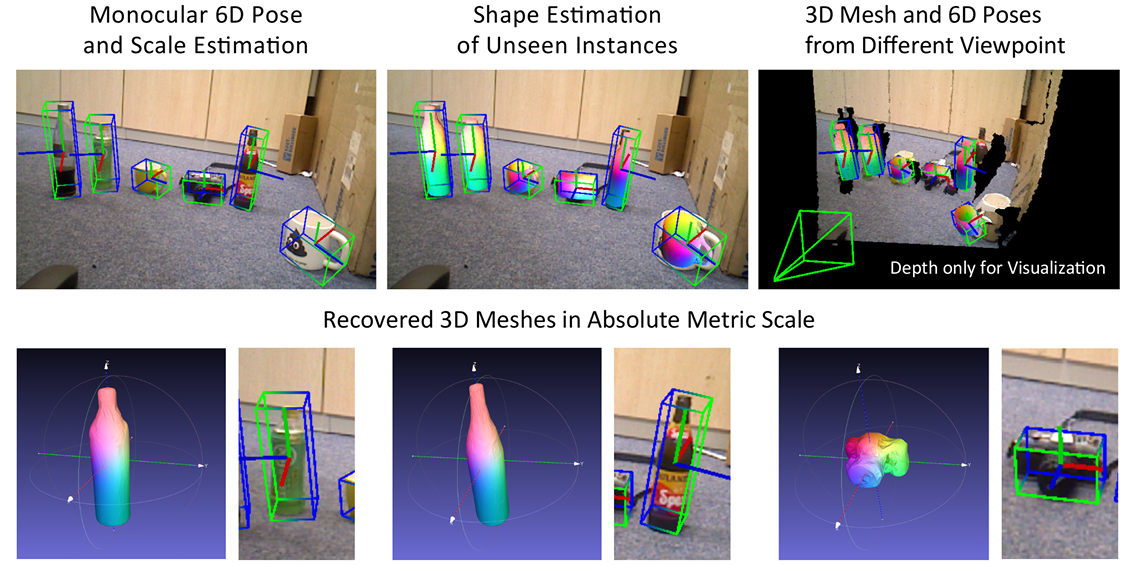
\includegraphics[width=0.95\linewidth]{figures/CPS++.png}
    \caption[CPS++: class-level 6D pose and shape estimation]{CPS++ \cite{manhardt2020cps++}: monocular RGB input (top left) with detected objects and estimated 6D pose and metric scale. Reconstructed 3D shapes are shown at the bottom, rendered into the scene (top center) and from an alternative viewpoint (top right) to verify consistent scale and alignment.}
    \label{fig:qual_real}
\end{figure}

\subsubsection{AI-Based Approaches}

End-to-end AI-based methods directly predict 6D pose from RGB or RGB-D inputs, often using convolutional neural networks (CNNs) or transformers. These models are more scalable and suitable for interactive or real-time deployment on modern hardware.

\paragraph{FoundationPose}

Among fully AI-based approaches, FoundationPose \cite{wen2024foundationpose} has recently drawn significant attention as a unified framework for 6D object pose estimation and tracking. It is designed to handle both model-based and model-free setups without requiring per-object fine-tuning, and achieves strong generalizability through a combination of large-scale synthetic training, large language model (LLM) guidance, a transformer-based architecture, and contrastive learning.

\begin{figure}[H]
    \centering
    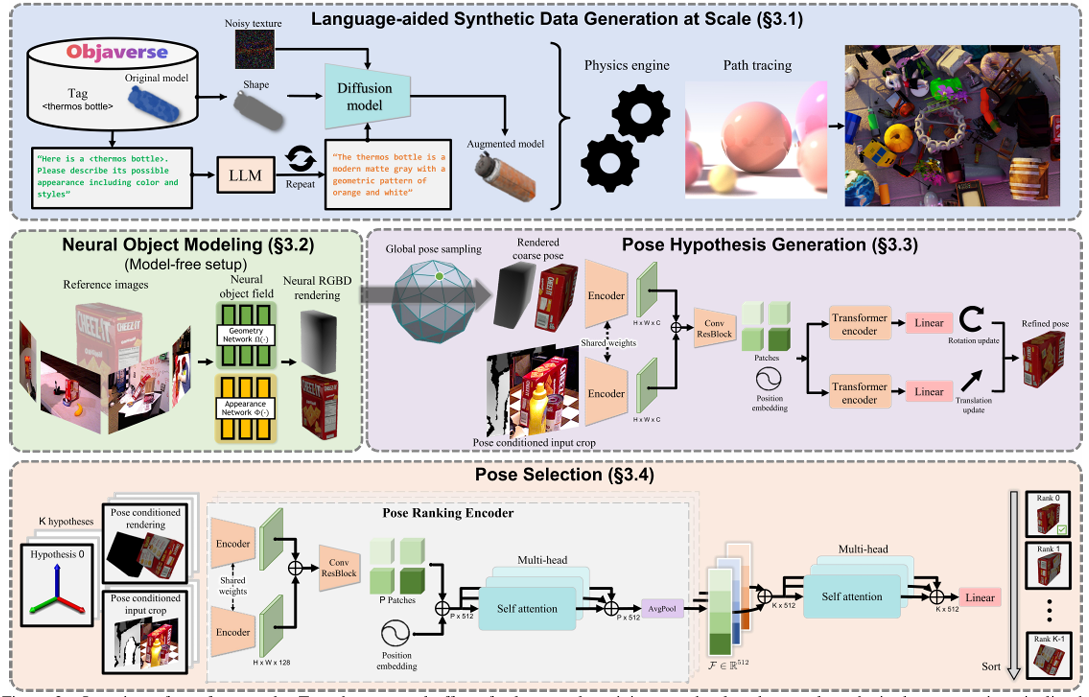
\includegraphics[width=\textwidth]{figures/foundationpose}
    \caption[FoundationPose pipeline overview]{Overview of the FoundationPose pipeline \cite{wen2024foundationpose}.}
    \label{fig:foundationpose_pipeline}
\end{figure}

The architecture of FoundationPose (Figure~\ref{fig:foundationpose_pipeline}) is organized into several key stages. Training begins with LLM-guided texture augmentation, where 3D models are drawn from large repositories such as Objaverse and Google Scanned Objects (GSO). Each model is assigned realistic textual descriptions generated by ChatGPT, which are then converted into diverse texture maps using the TexFusion diffusion model. The textured assets are inserted into randomized environments created with NVIDIA Isaac Sim, where object placement, illumination, and camera parameters are varied extensively. This pipeline produces more than 1.2~million high-quality synthetic RGB-D images for training, ensuring coverage of diverse visual conditions.  

In model-free settings, objects are represented through a neural signed distance function (SDF) paired with an appearance function. This representation is trained via volume rendering, where the network learns to match both geometry and appearance. The optimization process combines multiple supervisory signals, including color reconstruction for appearance fidelity, Eikonal regularization for smooth geometry, and near-surface constraints to sharpen the representation of object boundaries.  

At inference time, pose hypotheses are initialized from bounding box detections provided by a 2D detector such as Mask R-CNN. Depth information provides an initial estimate of translation, while multiple candidate rotations are sampled to cover the object’s orientation space. These hypotheses are then passed to the pose refinement network, a hybrid CNN–transformer architecture that follows a render-and-compare strategy. For each candidate, the network aligns a synthetic RGB-D rendering with the corresponding crop from the input frame and predicts iterative corrections to translation and rotation until convergence.  

Refined hypotheses are evaluated in the pose selection stage. Here, a hierarchical transformer performs two levels of comparison: locally, it assesses each hypothesis against the observation, and globally, it jointly considers all hypotheses to establish relative rankings. The best-scoring pose is chosen, and a contrastive triplet loss ensures that correct hypotheses are consistently ranked higher than incorrect alternatives.  

Finally, in tracking mode, temporal consistency is exploited by initializing the next frame from the previous frame’s pose estimate. This removes the need for fresh hypothesis generation, requiring only a single refinement step per frame. As a result, the system achieves around 32~frames per second on an RTX~3090 GPU, while maintaining robustness across both pose estimation and tracking scenarios \cite{wen2024foundationpose}.

Performance is reported with standard metrics: ADD (Average Distance of Model Points), ADD-S (symmetric ADD for symmetric objects), and AR (Average Recall used in the BOP benchmarks). FoundationPose was evaluated extensively on LINEMOD, Occluded-LINEMOD, YCB-Video, T-LESS, and YCBInEOAT, covering both pose estimation and tracking.

In the model-free setting on YCB-Video (Figure~\ref{fig:foundationpose_results}, left), FoundationPose reached 97.4\% ADD-S and 91.5\% ADD AUC, outperforming FS6D \cite{he2022fs6d} by a large margin and setting a new state-of-the-art. In the model-based evaluation on BOP benchmarks (Figure~\ref{fig:foundationpose_results}, right), it achieved an average recall of 83.3\%, surpassing instance-level methods such as MegaPose \cite{labbe2022megapose}. For pose tracking on YCB-Video, FoundationPose attained 93.7\% ADD and 97.5\% ADD-S AUC, showing robust performance in real-time operation \cite{wen2024foundationpose}.  

\begin{figure}[H]
    \centering
    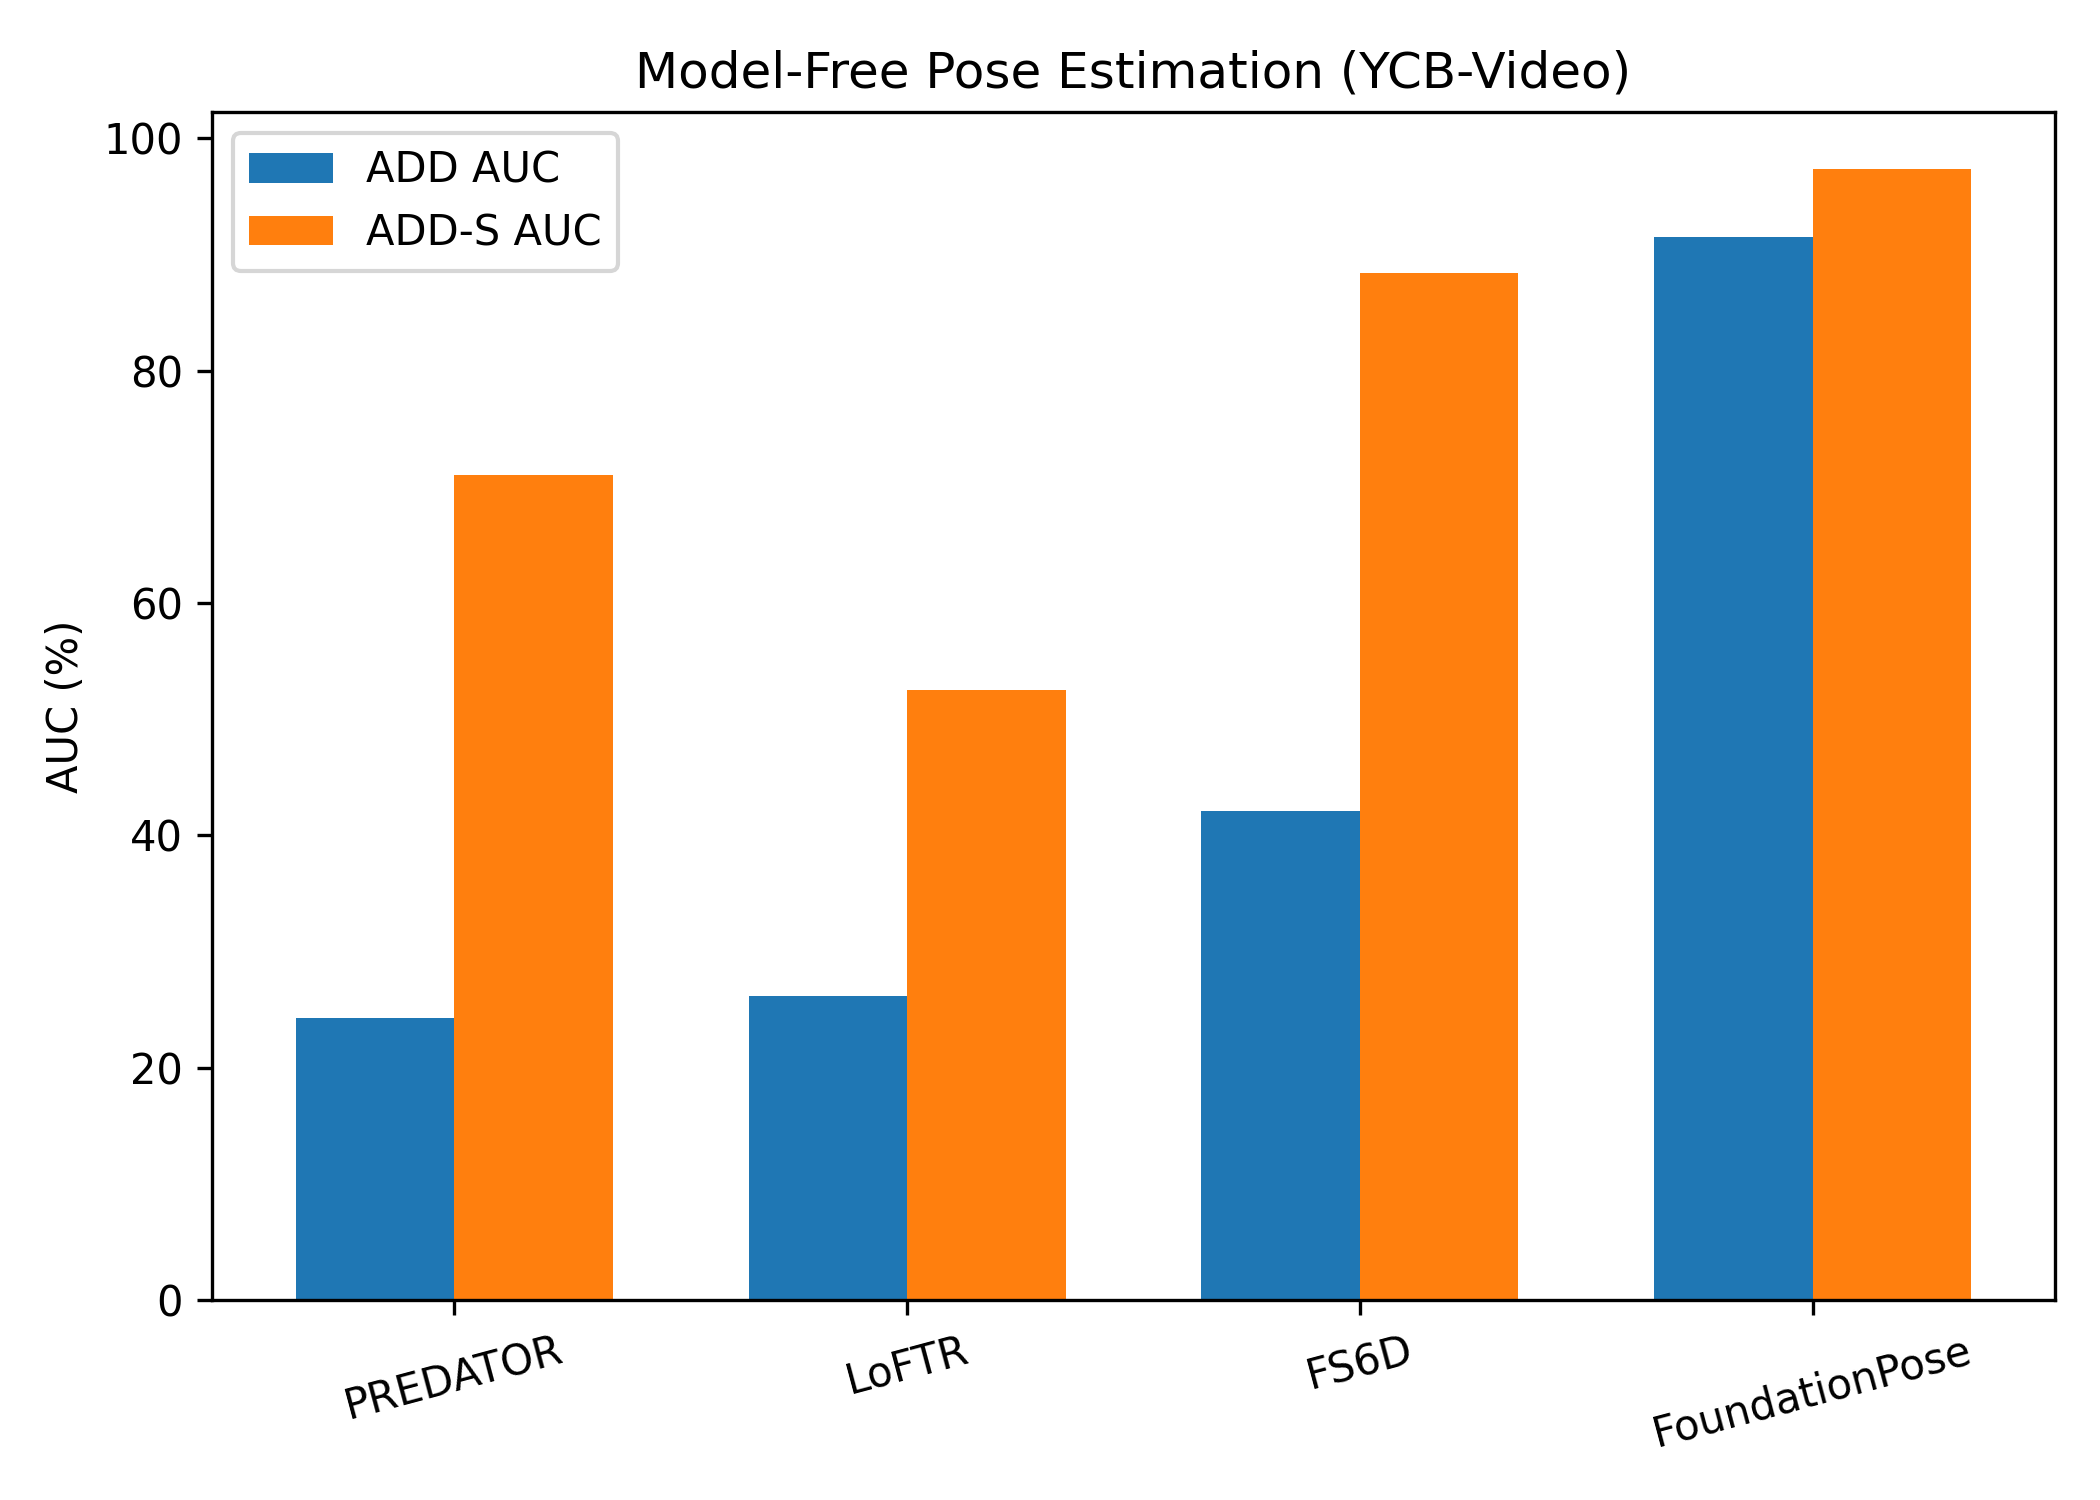
\includegraphics[width=0.48\textwidth]{figures/foundationpose_modelfree.png}
    \hfill
    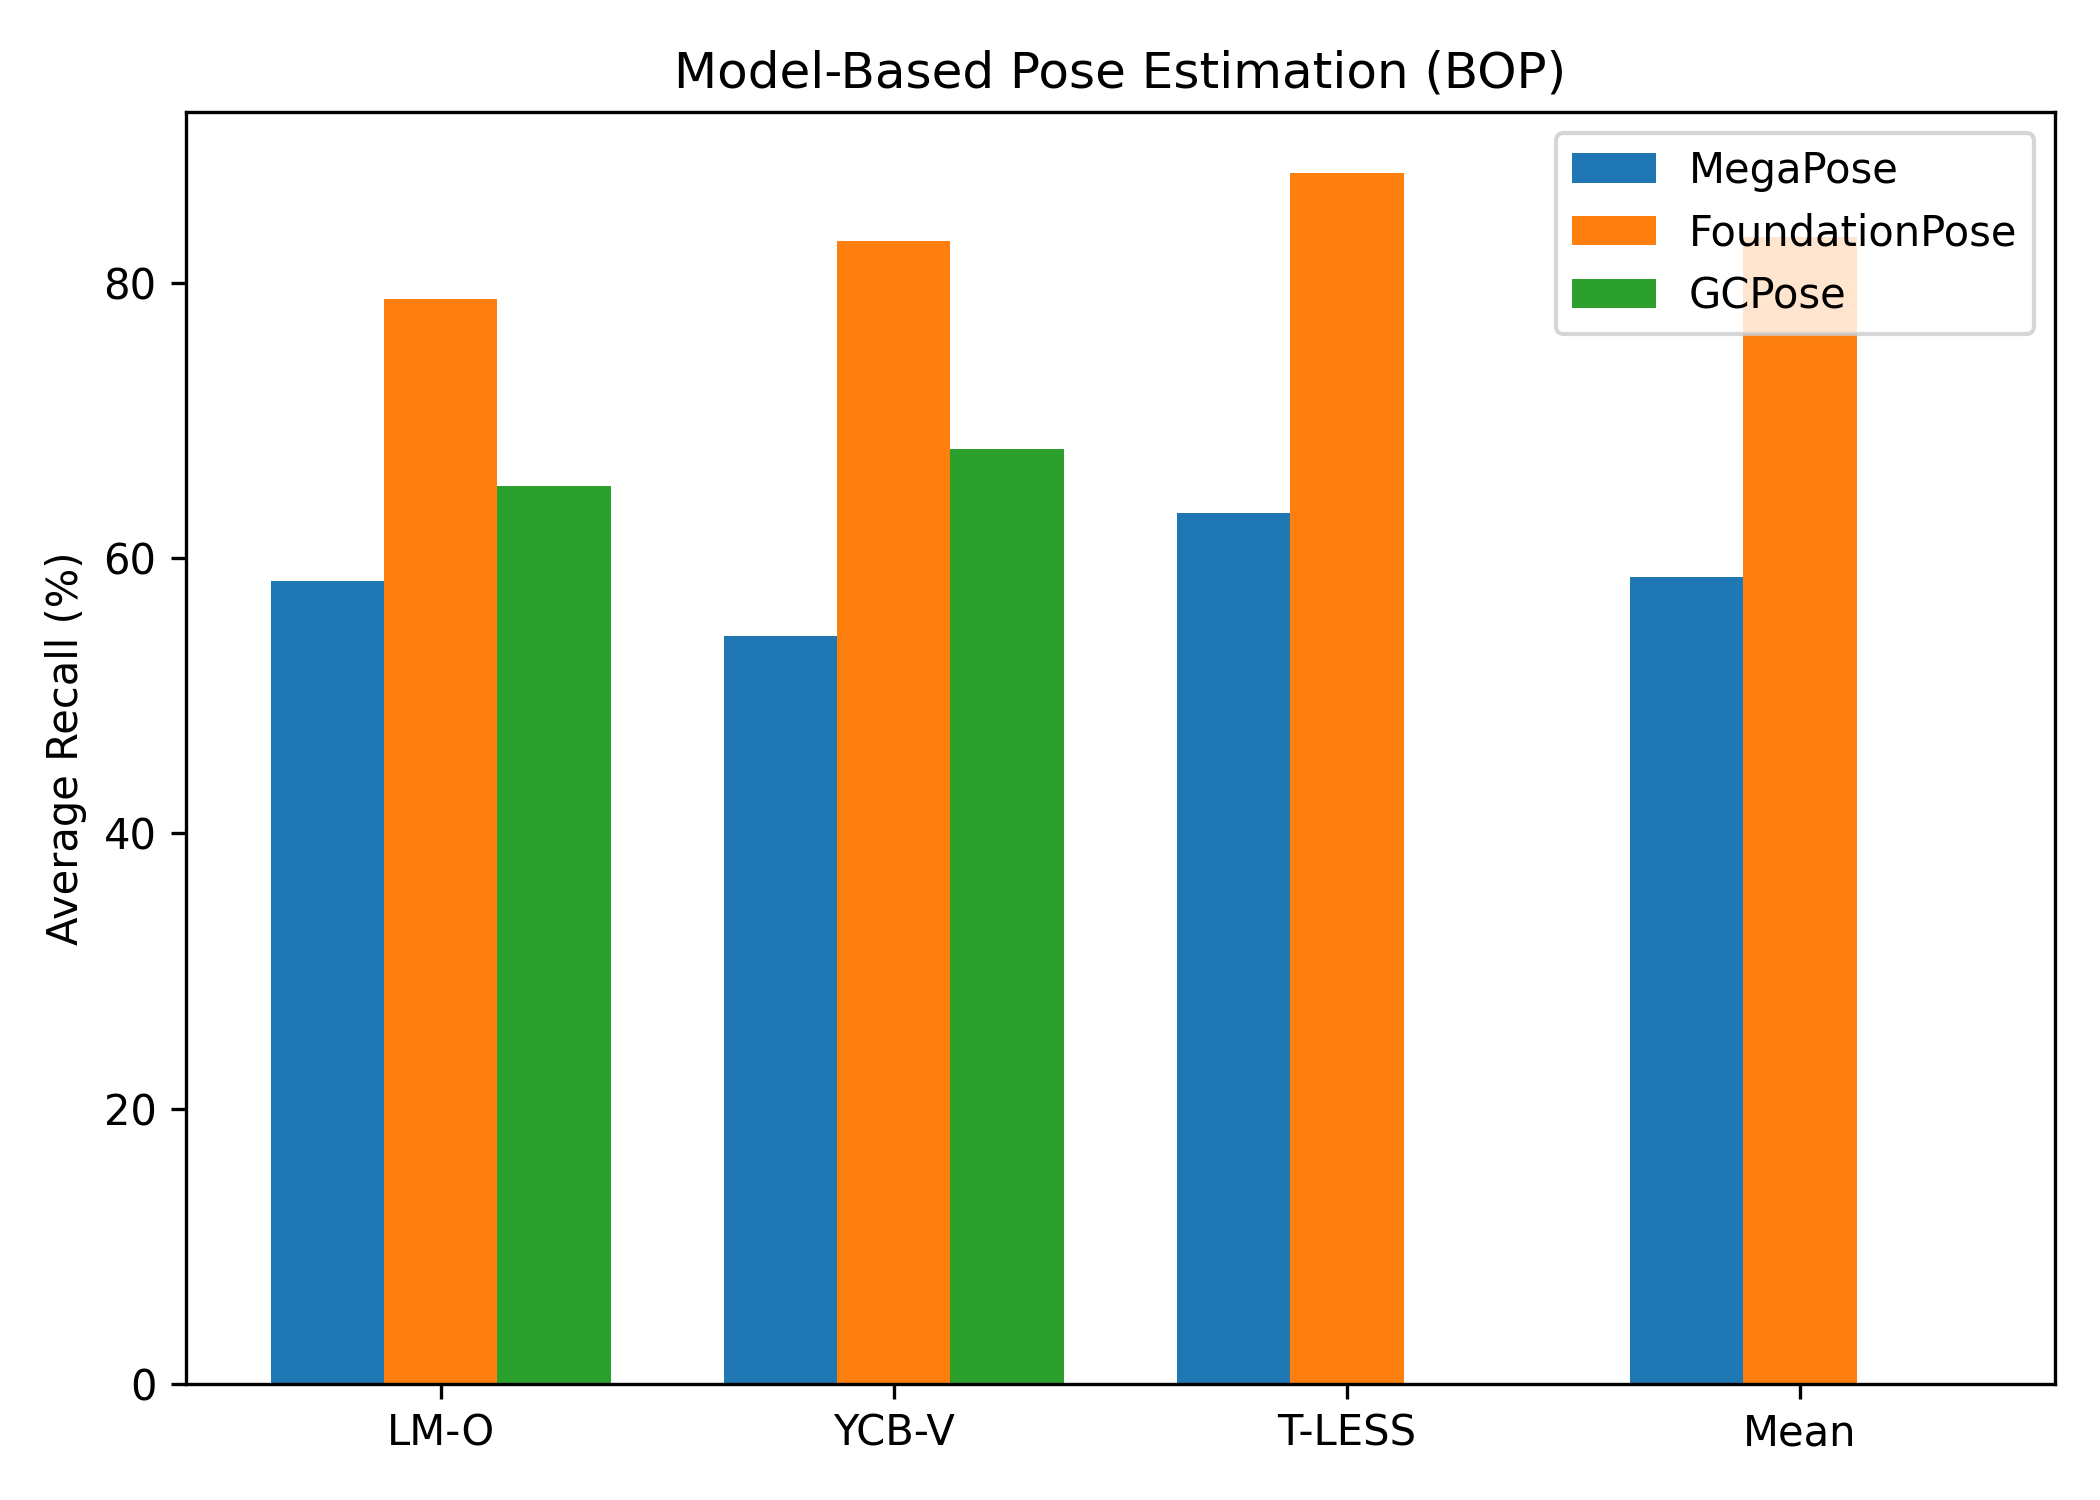
\includegraphics[width=0.48\textwidth]{figures/foundationpose_modelbased.png}
    \caption[FoundationPose evaluation on YCB-Video and BOP benchmarks]{Evaluation of FoundationPose \cite{wen2024foundationpose}. Left: model-free results on YCB-Video (ADD and ADD-S AUC). Right: model-based results on BOP benchmarks (Occluded-LINEMOD, T-LESS, YCB-Video).}
    \label{fig:foundationpose_results}
\end{figure}

Ablation experiments highlight the contribution of individual components. Removing LLM-based texture augmentation reduced ADD AUC from 91.5 to 90.8, replacing transformers with CNNs lowered it to 90.7, dropping hierarchical selection further reduced it to 89.1, and substituting the triplet loss with InfoNCE gave 89.4~\cite{wen2024foundationpose}. These results show that hierarchical ranking provides the largest performance gain. Additional scaling studies indicate that accuracy saturates at approximately twelve reference views and one million synthetic training scenes, suggesting diminishing returns beyond this point.

\paragraph{CNNPose}

Another influential method is CNNPose \cite{xiang2018posecnnconvolutionalneuralnetwork}, one of the earliest convolutional architectures designed for direct 6D pose estimation of known objects from RGB images. It addressed challenges in cluttered and occluded environments by decoupling translation and rotation estimation, moving away from 3D coordinate regression pipelines. Instead, it leveraged center localization, semantic segmentation, and region-specific feature pooling to provide robustness and generalization. This framework became a cornerstone for later approaches such as PoseCNN, DeepIM, and category-level methods.

\begin{figure}[H]
    \centering
    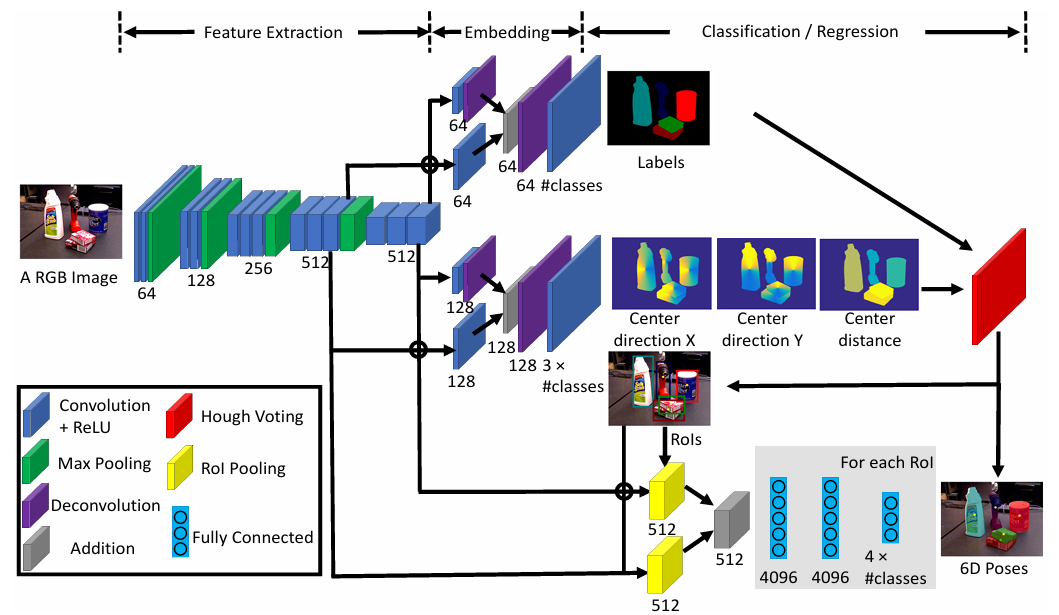
\includegraphics[width=\textwidth]{figures/posecnn.png}
    \caption[Architecture of CNNPose]{Architecture of CNNPose for 6D object pose estimation. The network performs semantic segmentation, center localization using Hough voting, and quaternion-based rotation regression \cite{xiang2018posecnnconvolutionalneuralnetwork}.}
    \label{fig:cnnpose}
\end{figure}

The architecture consists of a shared CNN backbone followed by three task-specific heads. The first branch performs semantic segmentation to classify pixels into object categories. The second branch estimates translation by regressing unit vectors toward object centers, which are aggregated with Hough voting to localize the 2D projection and reconstruct the 3D translation using depth. The third branch handles rotation estimation by applying region-of-interest (RoI) pooling over object regions and regressing the resulting features to a quaternion representation of orientation.  

To address symmetric objects, CNNPose introduced the \emph{ShapeMatch-Loss}, which compares object geometry via closest-point correspondences rather than penalizing orientation ambiguities. This proved especially effective on symmetric objects such as clamps and blocks. Alongside the method, the authors introduced the YCB-Video dataset, containing 92 RGB-D videos with 21 objects and over 133k annotated frames, which has since become a benchmark standard.

CNNPose was extensively evaluated on YCB-Video and OccludedLINEMOD using ADD and ADD-S metrics. On YCB-Video, CNNPose achieved 75.9\% AUC with RGB-only input and 93.0\% with ICP refinement, significantly outperforming 3D coordinate regression baselines. On OccludedLINEMOD, it achieved a mean accuracy of 24.9\% with RGB-only input, which increased to 78.0\% with ICP. These results demonstrated that center localization and symmetry-aware training provide robustness to heavy occlusion and object ambiguities (see Figure~\ref{fig:cnnpose_results}) \cite{xiang2018posecnnconvolutionalneuralnetwork}.  

\begin{figure}[H]
    \centering
    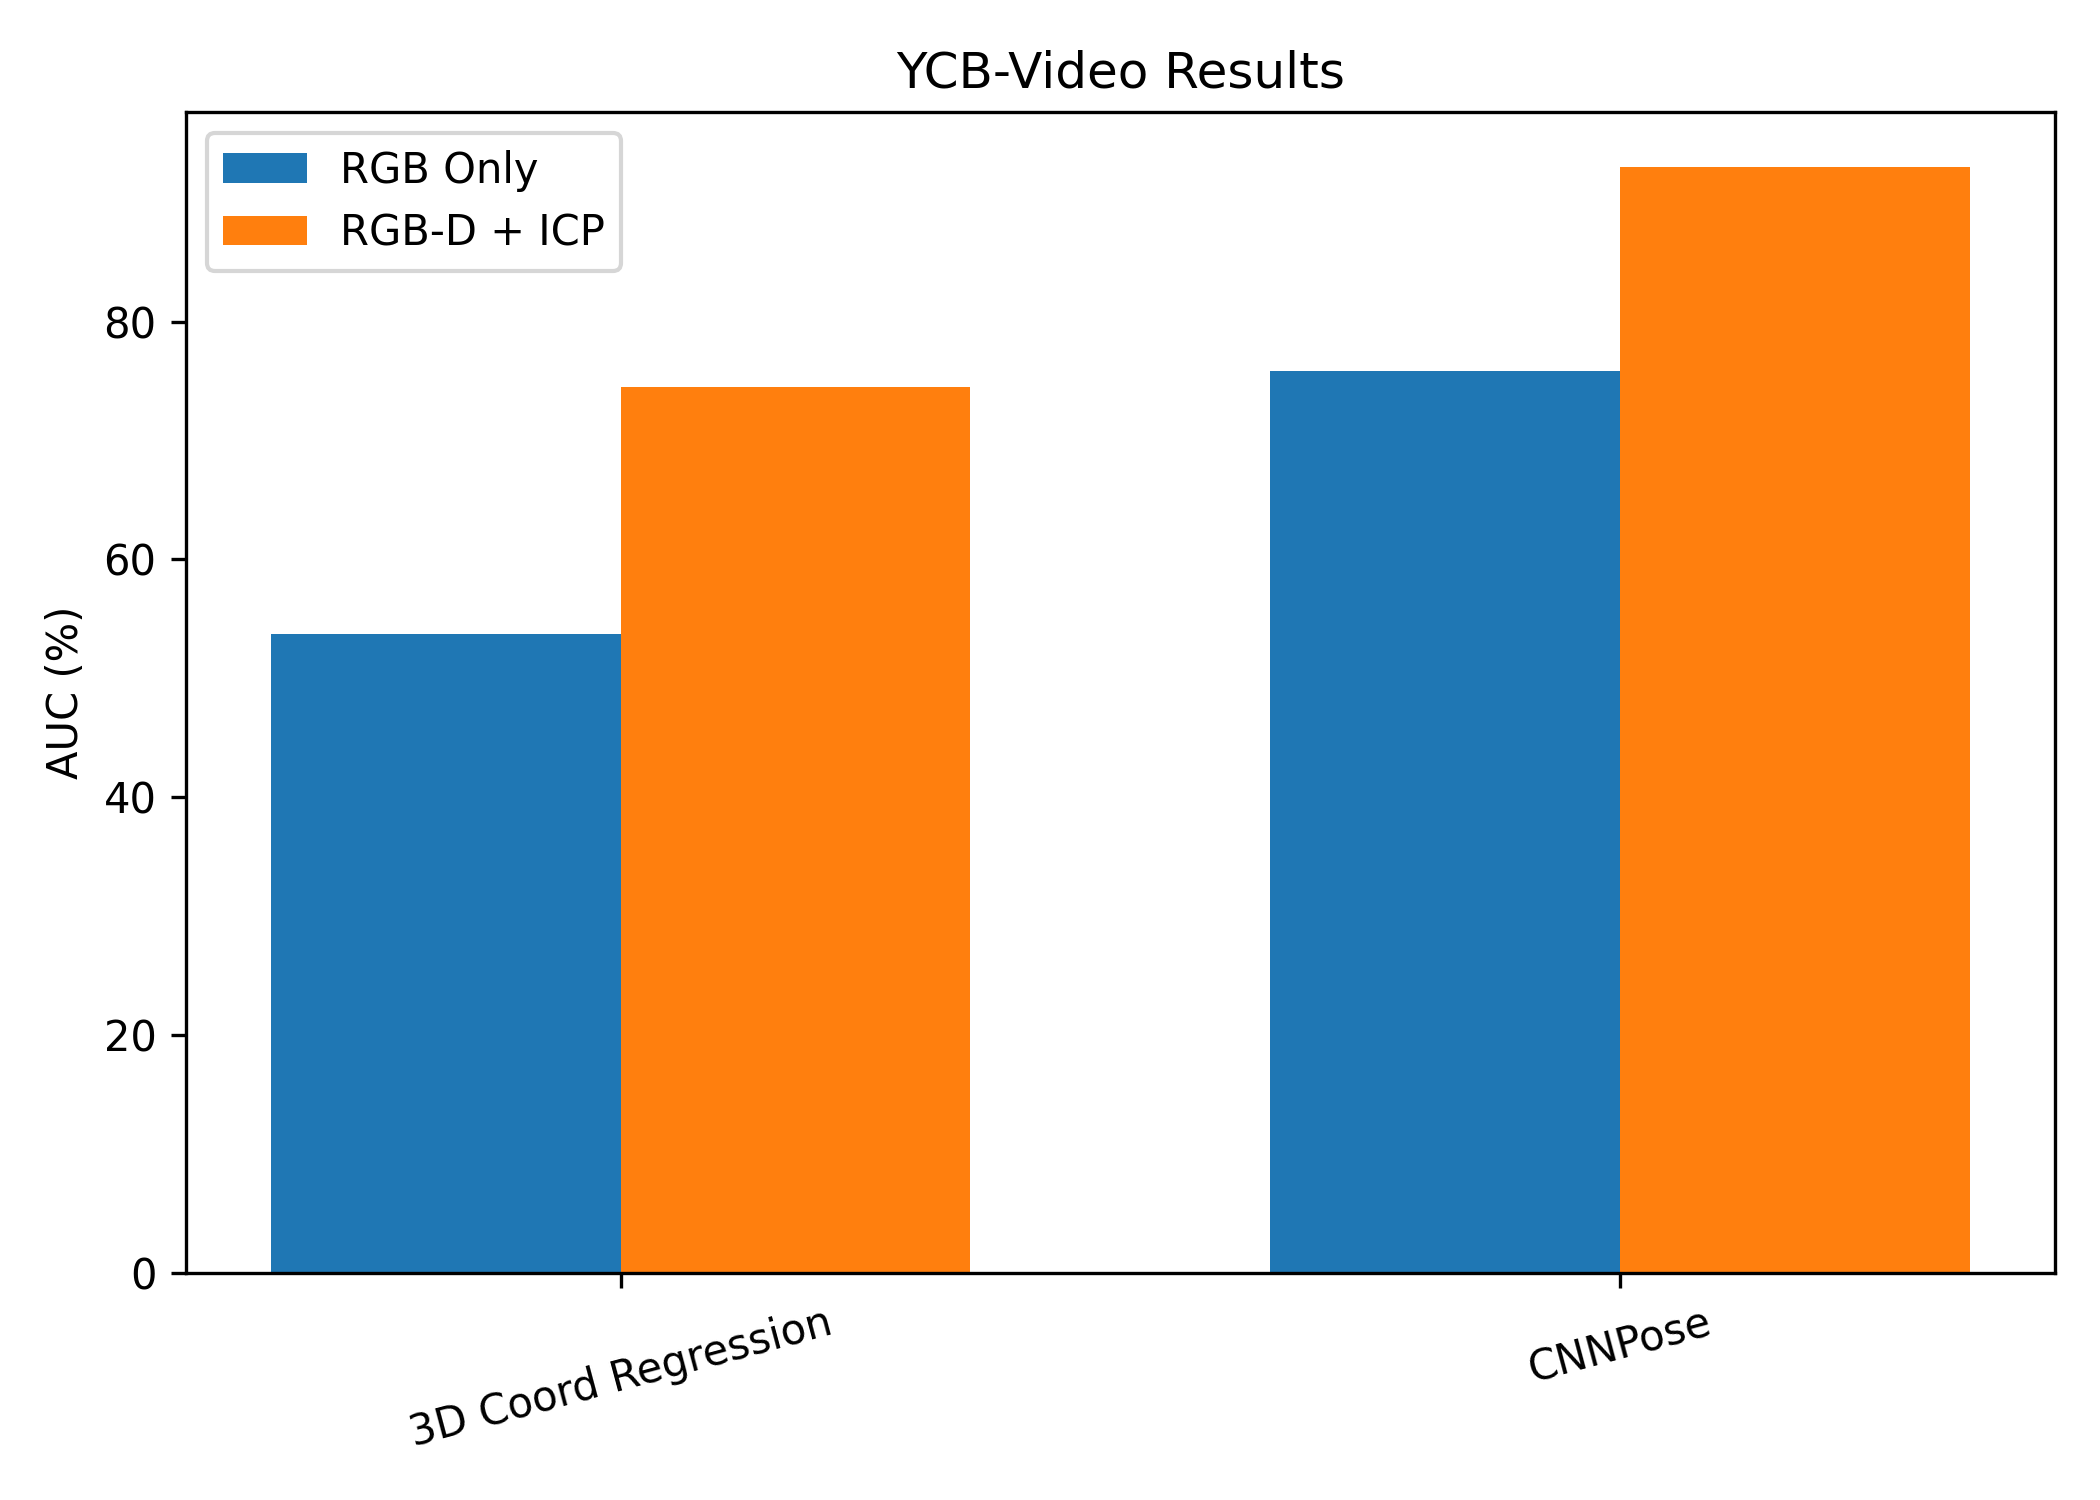
\includegraphics[width=0.48\textwidth]{figures/cnnpose_ycb_results.png}
    \hfill
    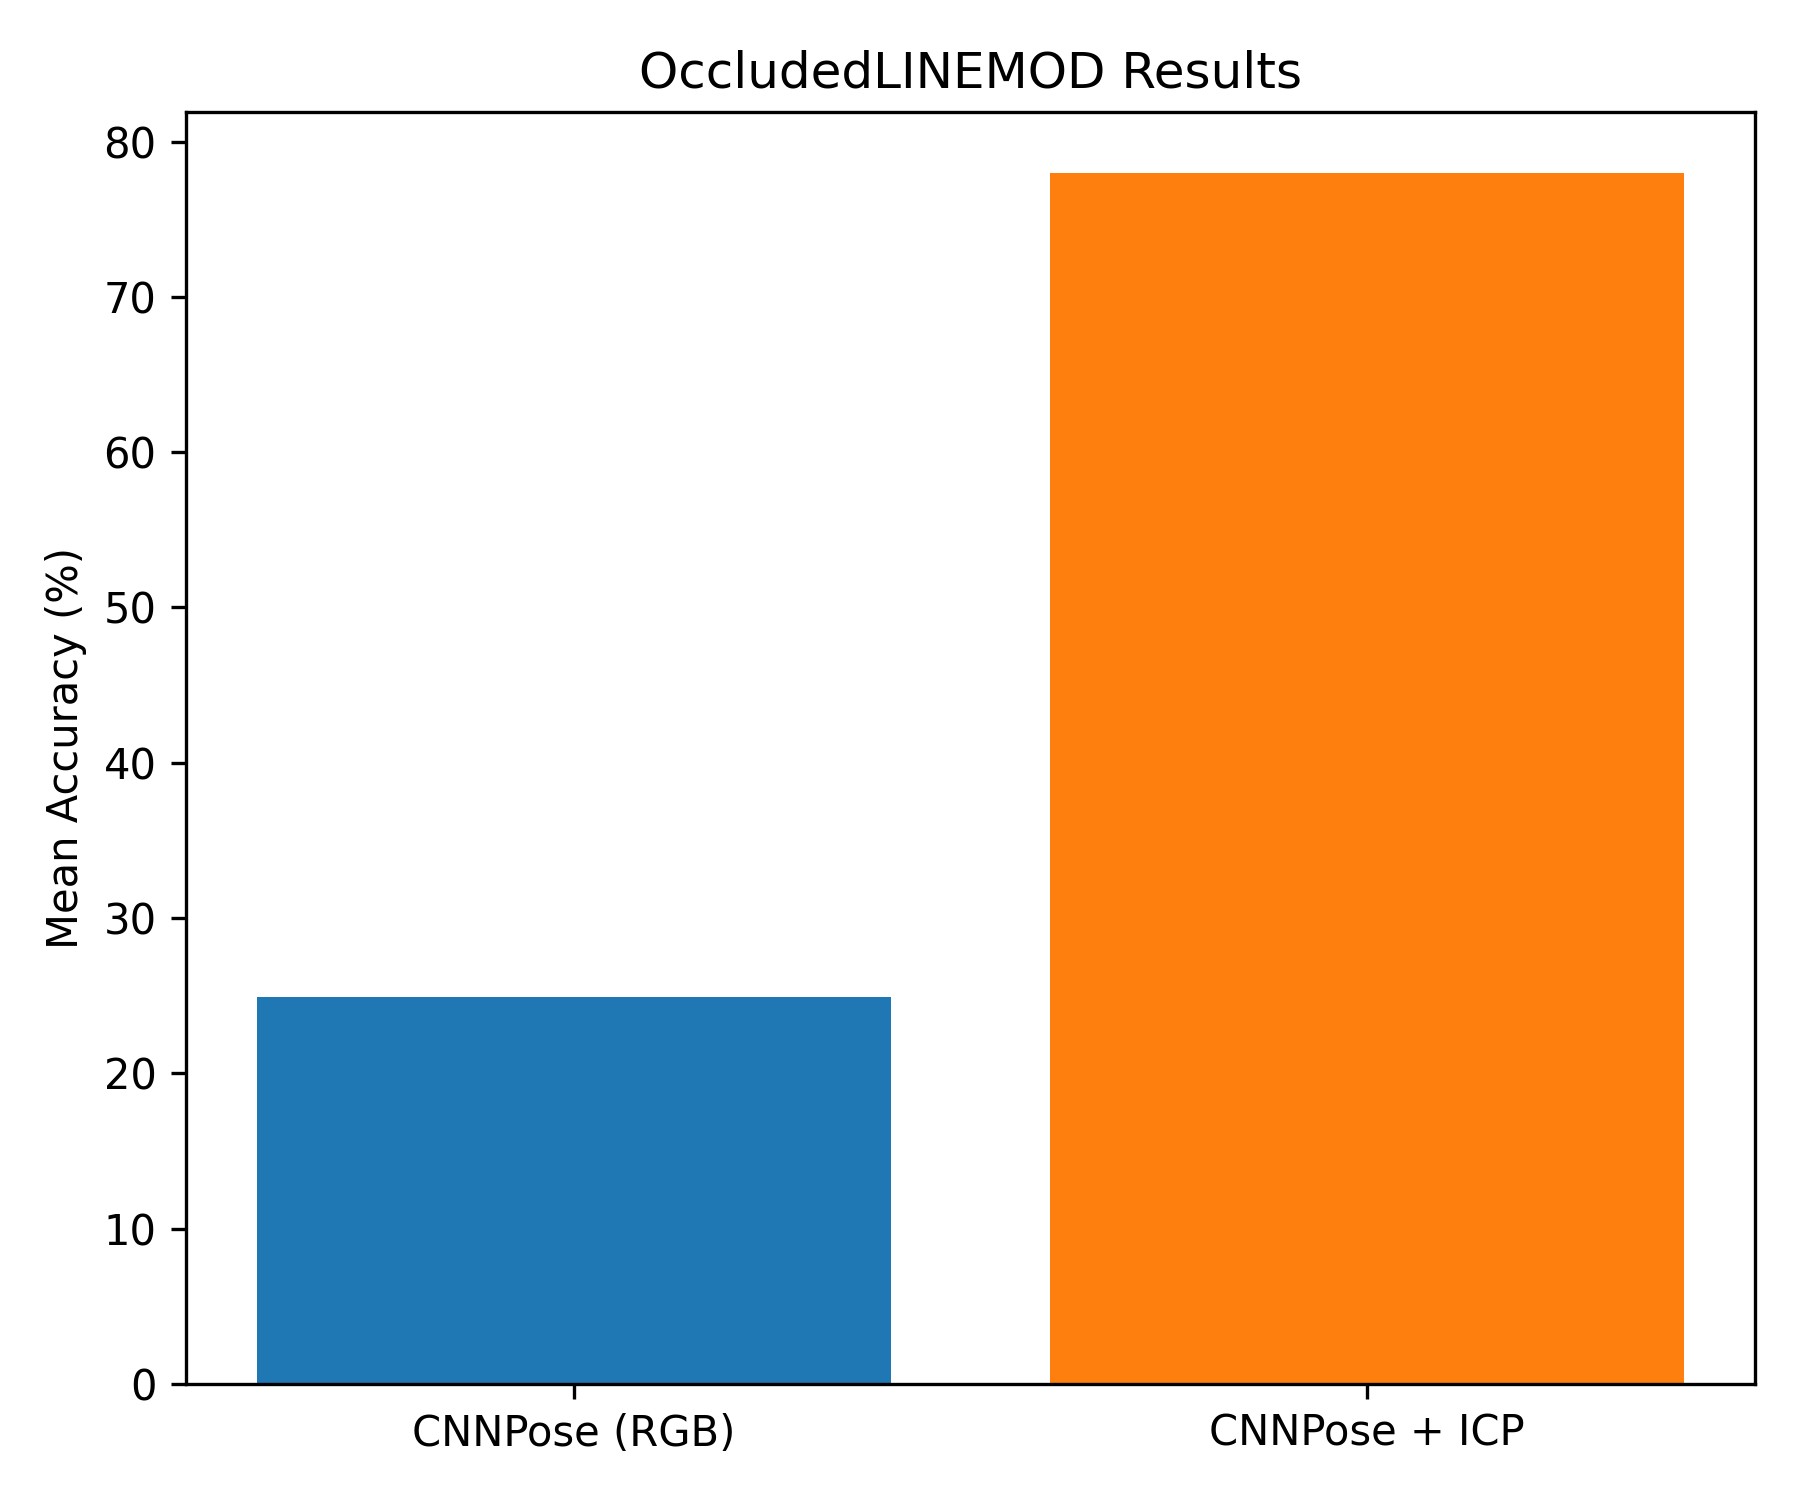
\includegraphics[width=0.48\textwidth]{figures/cnnpose_occluded_results.png}
    \caption[CNNPose performance on YCB-Video and Occluded-LINEMOD]{Performance of CNNPose \cite{xiang2018posecnnconvolutionalneuralnetwork}. Left: results on YCB-Video dataset (AUC). Right: results on Occluded-LINEMOD dataset (mean accuracy). ICP refinement yields substantial improvements, particularly under occlusion.}
    \label{fig:cnnpose_results}
\end{figure}

\paragraph{Occlusion-Aware Self-Supervised Pose Estimation}

The TUM team mentioned in Section~\ref{subsubsec:aiassisted} also proposed an occlusion-aware self-supervised framework for monocular 6D object pose estimation \cite{wang2021occlusion}. Their method begins with synthetic pretraining of an extended GDR-Net pose estimator and a refinement network. Both modules are trained exclusively on synthetic RGB data, ensuring a strong initialization without requiring annotated real-world labels. A YOLOv4 detector is also used in the pipeline to provide bounding boxes for object localization.  

After pretraining, the system adapts to real, unlabeled RGB(-D) images using a combination of noisy student training and differentiable rendering. In noisy student training, predictions from clean inputs serve as pseudo-labels to supervise outputs from augmented inputs, allowing the network to exploit large volumes of unlabeled data. Differentiable rendering further strengthens this adaptation by rendering RGB and depth images from predicted poses and comparing them with real sensor observations, enforcing both photometric and geometric consistency. As illustrated in Figure~\ref{fig:occlusionaware_selfsupervised}, this combination allows the network to bridge the gap between synthetic and real domains without relying on labeled data.  

A key innovation is the occlusion-aware mask prediction module, which estimates not only visible object regions but also amodal masks that approximate the full object extent under occlusion. This provides stability in cluttered environments, ensuring that pose refinement does not collapse when large parts of the object are hidden. The combination of self-supervised pseudo-labeling, rendering constraints, and occlusion handling enables the system to generalize effectively without requiring real pose annotations.  

\begin{figure}[H]
    \centering
    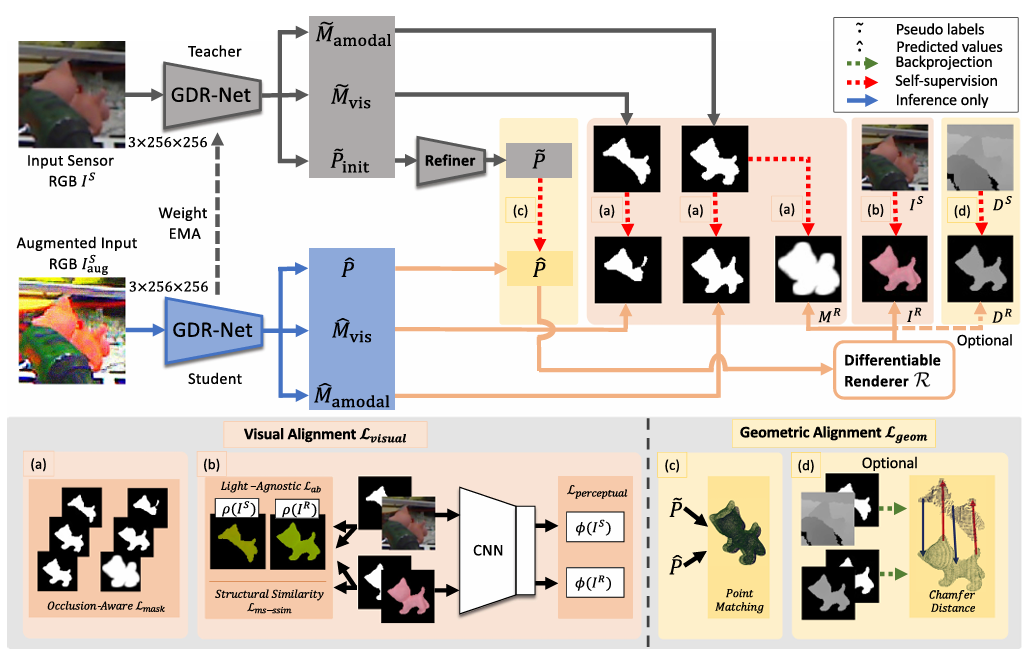
\includegraphics[width=\textwidth]{figures/occlusionaware_self_supervised.png}
    \caption[Occlusion-aware self-supervised 6D pose estimation]{Overview of occlusion-aware self-supervised framework for monocular 6D object pose estimation.ööö\cite{wang2021occlusion}.}
    \label{fig:occlusionaware_selfsupervised}
\end{figure}

This approach demonstrated state-of-the-art self-supervised results, reaching 91.1\% ADD-S AUC on YCB-Video and 40.8\% ADD AUC on Occluded-LINEMOD, surpassing previous methods such as Self6D (62.9\% and 21.0\%) and FS6D (88.4\% and 32.0\%) \cite{wang2021occlusion}, which shows good potential robustness of the framework in and occluded settings.
